% ============================================================
% experiments/exp02_selection_scale/report.tex
% exp02_selection_scale 实验报告 —— 第一阶段任务选择的规模压缩收益与标定口径
%
% 数据来源（路径均相对本文件）：
%   results/metrics.json   N × variant 扫描矩阵（17 格，唯一数值来源）
%   results/figures/      图产物（6 个：S01 + R01~R05）
%
% 编译：latexmk -xelatex report.tex     （ctex 需 xelatex）
% ============================================================
\documentclass[a4paper,11pt]{article}

\usepackage[margin=2.3cm]{geometry}
\usepackage{graphicx}
\usepackage{booktabs}
\usepackage{caption}
\usepackage{float}
\usepackage{amsmath,amssymb}
\usepackage{array}
\usepackage[table]{xcolor}
\usepackage[hidelinks]{hyperref}
\usepackage{ctex}
\usepackage{seqsplit}

\graphicspath{{results/figures/}}

% 长文件名/命令行：允许在任意字符间断行，避免 Overfull
\newcommand{\fname}[1]{{\ttfamily\seqsplit{#1}}}

\captionsetup{font=small,labelfont=bf,skip=6pt}
\setlength{\parskip}{4pt}
\renewcommand{\arraystretch}{1.15}
\setlength{\tabcolsep}{5pt}

\title{\textbf{exp02\_selection\_scale 实验报告}\\[6pt]
\large 动态任务分配两阶段框架：任务选择层的规模压缩收益与标定口径}
\author{}
\date{实验日期：2026--10--20\quad 随机种子：seed = 42\quad 扫描矩阵：3 规模 × 5 变体 + 全量对照}

\begin{document}
\maketitle

\begin{abstract}
\noindent 本报告记录 exp02\_selection\_scale 实验的设置与结果。实验针对
Chapter3\_README \S 1(4) 的待验证命题——当 $|T_t| \gg K$ 时，
第一阶段「动态任务选择」的候选压缩（$n_{\mathrm{cand}}=\lceil\alpha K\rceil$）能否提高实时性——在真实 DEM 地形
（SRTM/ASTER 级高程数据，200\,m 采样）上固定 $K=8$、满电航程
80\,km，将任务规模扫到 50/100/200，并对两种规模标定口径（机数名额族
\texttt{quota\_*} vs 机队能力驱动族 \texttt{cap\_x*}）做 17 格对照扫描。
结果显示：(1)~压缩真实发生且与 $N$~\textbf{解耦}——候选数恒为
20/40 或 $\mathrm{cap}(t)=10/20/40$，不随任务规模变化；
(2)~第二阶段耗时与 $N$~\textbf{无关}（固定 $n_{\mathrm{sel}}=16$ 时 25.3/25.2/25.0\,s，
三次测量极差 $<2\%$）；(3)~原结论「$\alpha$ 需按机队总吞吐标定」被修正为
更精确的答案——intersect 口径下\textbf{真正瓶颈是选择数
$n_{\mathrm{sel}}=\lceil \mathrm{max\_ratio}\cdot K \rceil = 16$ 而非 $\alpha$}
（\texttt{quota\_a2.5} 与 \texttt{quota\_a5} 结果几乎相同）；
(4)~能力驱动口径（选择数接到 $\mathrm{cap}(t)$）把压缩损失大部分买回来：
$n_{\mathrm{sel}} \approx \mathrm{cap}(t)$ 时 F1 达全量的 93.5\%（$N{=}50$）/ 83.4\%（$N{=}100$），
而耗时仅为其 87\%/13\%（$N{=}100$ 加速 7.6$\times$），$\mathrm{cap}(t)$ 即
「质量—耗时」的天然平衡点。实验同时验证了代价矩阵延迟构建（惰性表）的效果：
$N{=}200$ 时一阶段仅现算 2,164 条边（全量的 5.0\%），端到端 $O(n^2)$ 构建占比
从旧版 85.6\% 降到 3.7\%。
\end{abstract}

\tableofcontents
\newpage

% ============================================================
\section{实验设置}
% ============================================================

\subsection{实验目标与评价口径}

本实验验证两阶段分层框架中\textbf{第一阶段（动态任务选择）的规模压缩机制}，
对应论文 Chapter3\_README \S 1(4) 与 \S 3.3。待验证命题：

\begin{quote}
当 $|T_t| \gg K(t)$ 时，把全部任务直接交给精细组合优化会显著扩大
搜索空间；第一阶段用 $n_{\mathrm{cand}}=\lceil\alpha K\rceil$ 把 $T_t$ 压到 $T_t^{\mathrm{sel}}$，
据称能提高实时性。
\end{quote}

\texttt{exp01\_smoke} 跑在「机多任务少」一侧（10 任务 / 24 机，$\lceil\alpha K\rceil = 60$），
$n_{\mathrm{cand}}$ 截断从不触发，无法验证该机制。本实验固定 $K = 8$
（8 巢 × 容量 4），把任务规模拉到 50/100/200，测量四个量：

\begin{itemize}
  \item $T_{\mathrm{hint}}$：\texttt{cost\_hint}（最近可用机，惰性表 $O(n \cdot K)$ 条边）；
  \item $T_{\mathrm{sel}}$：第一阶段耗时 + 压缩率 $|T_t| \to |T_t^{\mathrm{sel}}|$；
  \item $T_{\mathrm{build}}$：候选子集三维矩阵构建（与一阶段共享惰性表缓存）；
  \item $T_{\mathrm{muas}}$：第二阶段对候选集求解的耗时。
\end{itemize}

由此回答三个问题：(1)~压缩是否真的发生了？压到多少？
(2)~分层省下的搜索时间，是否被 $O(n^2)$ 代价构建吃掉？
(3)~候选规模按「机数名额」还是「机队能力」标定，吞吐—耗时—质量的平衡点在哪里？

\textbf{指标口径（2026-10-22 v2）}：报告层的完成/按时/成本类指标一律采用
论文主表 v2 口径——最终完成率 $\eta_{\mathrm{final}}$（分母排除物理不可达、
保留超期淘汰）、按时率（最终交付口径，迟到计完成不计按时）、
单位完成航程 $=$ 总航程（含返航）/完成数；过程指标含名额利用率
$\sum n_{\mathrm{sel}}^{\mathrm{used}}/\sum n_{\mathrm{sel}}^{\mathrm{cap}}$
与跨周期推迟量，方法诊断含 $n_{\mathrm{skip}}$ / 一阶 shortfall 分账
（定义详见 \fname{exp01\_smoke/report.tex} \S 1.2）。

\subsection{实验定位与证据边界}

本实验属\textbf{L2 设计有效性}证据：验证「选择层压缩」这一设计在
$|T_t| \gg K$ 规模下真实有效、且给出标定口径。本报告\textbf{可以}声称：
压缩机制按协议工作（四项目标标准全部达成，见 \S 2.2）、两种标定口径的
权衡曲线可定位、$O(n^2)$ 构建瓶颈已被延迟构建消除。本报告\textbf{不能}声称：

\begin{itemize}
  \item \textbf{方法优于任何基线}——对比方法尚未接入统一评价（属 exp05 职责）；
        本实验的「全量对照」（不经过第一阶段直接全量求解）是\textbf{同一求解器}
        的质量上界参照，不是方法学基线；
  \item \textbf{单 seed 稳健性}——仅 seed 42；多种子稳健性未做
        （exp01 侧已做 3 seed）；
  \item \textbf{生产级解质量}——求解预算为 40 代 + 800 评估（exp01 生产为
        100 代 + 2000），本实验量的是权衡曲线\textbf{形状}，各格同预算、横向可比；
  \item \textbf{$N{=}200$ 的质量上界}——全量对照单格求解约 25\,min、代价不成比例，
        未测；该规模的「无压缩上界」由 $N{=}50/100$ 的损失比例外推说明
        （机制不随 $N$ 变，结论 2 已证明耗时与 $N$ 无关）。
\end{itemize}

\subsection{场景与地形}

复用 exp01\_smoke 的场景口径：实验区域位于青藏高原（约 N29$^\circ$/E091$^\circ$），
高程数据取自 \fname{ASTGTMV003\_N29E091\_dem.tif}，采样步长 200\,m，
8 个机巢，场景范围约 $101.6 \times 115.0$\,km。

\textbf{距离口径}：所有距离一律采用\textbf{垂直切面 DEM 三维航程}，
凡由距离推导时间（ETA、时间窗判定、航程约束、边际插入估计）均由统一的
代价提供者计算，保证全链路口径一致。

\textbf{机群构型（2026-10-20 修复项）}：无人机按 exp01 \fname{build\_uavs} 口径
\textbf{驻留其机巢}（UAV $i \to$ 巢 $i \bmod 8$），满电航程 80\,km。
旧版把全部 UAV 放在局部平面原点，最近可用机距离中位数被推到 39.4\,km、
$\mathrm{cap}(t)$ 缩到 16、24/50 个任务被往返预筛误杀——整个规模实验测的是
「原点邻域」这个退化构型。驻巢修复后：中位距离 15.2\,km、
$\mathrm{cap}(t) \approx 41$、预筛零误杀，与全量对照的执行数同量级。

\subsection{变体矩阵：两种规模标定口径}

扫描矩阵固定任务生成参数（锚定机巢撒点、spread 25\,km、奖励 $1 \sim 10$、
时间窗 $1 \sim 8$\,h），只变「候选/选择规模政策」：

\begin{table}[H]
\centering
\caption{变体矩阵（两个标定族 + 全量对照）}
\label{tab:variants}
\small
\begin{tabular}{@{}lllll@{}}
\toprule
变体 & 族 & $\alpha$ & capability 模式 & 含义 \\
\midrule
\texttt{quota\_a2.5} & 名额族 & 2.5 & intersect（收紧） & $n_{\mathrm{cand}} = \lceil \alpha K \rceil = 20$ \\
\texttt{quota\_a5}   & 名额族 & 5.0 & intersect（收紧） & $n_{\mathrm{cand}} = \lceil \alpha K \rceil = 40$ \\
\texttt{cap\_x0.25}  & 能力族 & 2.5 & primary（定规模）  & 规模 $= \mathrm{cap}(t) \approx 10$ \\
\texttt{cap\_x0.5}   & 能力族 & 2.5 & primary（定规模）  & 规模 $= \mathrm{cap}(t) \approx 20$ \\
\texttt{cap\_x1}     & 能力族 & 2.5 & primary（定规模）  & 规模 $= \mathrm{cap}(t) \approx 40$ \\
\texttt{full\_baseline} & 对照 & --- & --- & 不经过第一阶段，全量 $N$ 直接求解 \\
\bottomrule
\end{tabular}
\end{table}

两种口径的本质差异：

\begin{itemize}
  \item \textbf{机数名额族（旧口径）}：候选规模 $n_{\mathrm{cand}} = \lceil \alpha K \rceil$ 只跟
        \emph{机器数}走，与机队吞吐能力脱钩；capability 以 \texttt{intersect}
        模式只能收紧不能放宽；
  \item \textbf{机队能力驱动族（待评口径）}：规模由
        \[
          \mathrm{cap}(t) = \left\lfloor \mathrm{budget\_scale} \cdot
          \frac{B}{\tilde{c}} \right\rfloor
        \]
        决定，其中 $B$ 为机队总航程（$8 \times 80\,\mathrm{km} = 640$\,km）、
        $\tilde{c}$ 为最近可用机三维航程中位数（驻巢修复后约 15\,km），
        $\mathrm{budget\_scale} \in \{0.25, 0.5, 1.0\}$；capability 以
        \texttt{primary} 模式\textbf{直接定规模}，机数名额只作兜底。
        实测 $\mathrm{cap}(t) = 41/40/40$（$N = 50/100/200$）。
\end{itemize}

\subsection{求解预算与计时口径}

\begin{itemize}
  \item \textbf{求解预算}（全格同口径）：DMDE 种群 20 × 40 代；
        polish $\le 20$ 轮 / $\le 800$ 评估；
  \item \textbf{计时}：\texttt{perf\_counter} 分段计时
        （hint / selection / build / muas），$T$ = 端到端四项之和；
  \item \textbf{惰性边数}：\texttt{LazyPairwiseCost} 实际现算边数
        （按需估算 + 缓存，值与全量 eager 建表\textbf{逐位一致}，
        已用旧代码 git stash 对照 + 非对称估算器方向单测双重验证）；
  \item \textbf{质量指标}：F1 = \texttt{f1\_reward}（按迟到折减后的交付收益），
        F2 = \texttt{f2\_cost}（路径代价，含返航腿）；
  \item \textbf{记录口径备注}：本版 \texttt{metrics.json} 的 \texttt{muas.n\_evals}
        字段误取了 diagnostics 字典键（该字典无此键，恒录 0），已修 \fname{run.py}
        改取 \texttt{MUASStageResult.n\_evals} 属性；本报告的评估数以 DMDE
        构造值（pop×gens = 800 + 灭绝重评）与 \texttt{polish\_evals} 列为准。
\end{itemize}

% ============================================================
\section{主要结果}
% ============================================================

\subsection{实测总表}

\begin{table}[H]
\centering
\caption{实测结果（seed = 42；$K=8$；$B = 8 \times 80\,\mathrm{km} = 640$\,km；$\mathrm{cap}(\times 1.0) \approx 41$）}
\label{tab:main}
\footnotesize
\setlength{\tabcolsep}{3.5pt}
\begin{tabular}{rrlrrrrrrrrr}
\toprule
N & 变体 & cap($t$) & 候选$n_{\mathrm{cand}}$ & $n_{\mathrm{sel}}$ & exec & F1 & F2(km) & $T$/s & muas/s & edges & pol \\
\midrule
50 & \texttt{quota\_a2.5} & 41 & 20 & 16 & 16 & 133.2 & 162.1 & 25.9 & 25.3 & 964 & 625 \\
50 & \texttt{quota\_a5}   & 41 & 40 & 16 & 16 & 129.1 & 151.8 & 27.3 & 26.5 & 1544 & 601 \\
50 & \texttt{cap\_x0.25}  & 10 & 10 & 10 & 10 &  89.8 & 147.6 & 10.7 & 10.4 & 644 & 296 \\
50 & \texttt{cap\_x0.5}   & 20 & 20 & 20 & 20 & 164.8 & 224.1 & 43.1 & 42.6 & 1024 & 800 \\
50 & \texttt{cap\_x1}     & 41 & 41 & 41 & 39 & 273.7 & 568.9 & 141.1 & 139.5 & 2473 & 800 \\
50 & \textbf{full}        & --- & 50 & 50 & 45 & \textbf{292.7} & 603.7 & 161.8 & 160.6 & 3364 & 800 \\
\midrule
100 & \texttt{quota\_a2.5} & 40 & 20 & 16 & 16 & 131.0 & 196.5 & 25.9 & 25.2 & 1364 & 359 \\
100 & \texttt{quota\_a5}   & 40 & 40 & 16 & 16 & 120.1 & 172.6 & 30.7 & 29.7 & 1944 & 703 \\
100 & \texttt{cap\_x0.25}  & 10 & 10 & 10 & 10 &  84.0 & 132.0 & 11.5 & 11.1 & 1044 & 135 \\
100 & \texttt{cap\_x0.5}   & 20 & 20 & 20 & 20 & 165.2 & 257.9 & 41.3 & 40.7 & 1424 & 800 \\
100 & \texttt{cap\_x1}     & 40 & 40 & 40 & 40 & 297.3 & 523.3 & 140.0 & 138.5 & 2784 & 800 \\
100 & \textbf{full}        & --- & 100 & 100 & 60 & \textbf{356.5} & 630.3 & 1068.5 & 1064.3 & 11664 & 800 \\
\midrule
200 & \texttt{quota\_a2.5} & 40 & 20 & 16 & 16 & 132.6 & 180.0 & 26.0 & 25.0 & 2164 & 513 \\
200 & \texttt{quota\_a5}   & 40 & 40 & 16 & 16 & 135.2 & 197.3 & 24.8 & 23.5 & 2744 & 581 \\
200 & \texttt{cap\_x0.25}  & 10 & 10 & 10 & 10 &  84.6 &  98.1 & 12.1 & 11.4 & 1844 & 257 \\
200 & \texttt{cap\_x0.5}   & 40 & 20 & 20 & 20 & 167.6 & 234.0 & 41.9 & 41.0 & 2224 & 800 \\
200 & \texttt{cap\_x1}     & 40 & 40 & 40 & 40 & 336.7 & 496.6 & 119.6 & 117.8 & 3584 & 800 \\
\bottomrule
\end{tabular}
\end{table}

口径：$T$ = 端到端（hint + sel + build + muas）；edges = 惰性表实际现算边数；
pol = polish 实际消耗评估数（800 即触顶，说明该格搜索仍有改进空间、被预算截断）。
漏斗（全部格子一致）：$N \to \mathrm{Top}\text{-}k \to k \to k$——驻巢修复后
往返预筛与 postcheck 均零拒绝（$2 \times 25$\,km 散布 $\le 80$\,km 航程），
规模完全由候选/选择数决定，\texttt{filter\_reasons} 只剩 \texttt{not\_in\_top\_alpha}。

\subsection{结论}

\textbf{四项目标标准全部达成，且标定口径的答案比原结论更精确：}

\begin{enumerate}
  \item \textbf{压缩真实发生且与 $N$ 解耦。} 名额族候选数恒为 20（$\alpha = 2.5$）
        或 40（$\alpha = 5$），不随 $N$ 变化；压缩比 $3.1\times \to 6.3\times \to 12.5\times$
        （$\alpha = 2.5$）随 $N$ 线性增长。能力族 $\mathrm{cap}(t) = 10/20/40$
        由 $B/\tilde{c}$ 决定，同样与 $N$ 无关（41/40/40）。
  \item \textbf{第二阶段耗时与 $N$ 无关（固定 $n_{\mathrm{sel}}$）。} $n_{\mathrm{sel}} = 16$ 时 muas
        25.3/25.2/25.0\,s（$N = 50/100/200$），三次测量极差 $< 2\%$；
        耗时只随 $n_{\mathrm{sel}}$ 涨（$n_{\mathrm{sel}}: 10 \to 41$ 时 $10.4 \to 139.5$\,s）。
  \item \textbf{延迟构建后 $O(n^2)$ 瓶颈消失。} $N = 200$：hint 0.57\,s +
        sel 0.32\,s + build 0.07\,s = 0.96\,s（占端到端 3.7\%），而旧版
        全量建矩阵一项就要 9.8\,s（占 85.6\%）。惰性表现算边数为全量的
        5.0\%（2,164/43,264）。端到端耗时现在由二阶段求解主导（96\%），
        这正是分层要保护的对象。
  \item \textbf{规模标定的真正瓶颈不是 $\alpha$，是选择数
        $n_{\mathrm{sel}}=\lceil \mathrm{max\_ratio} \cdot K \rceil = 16$。}
        \texttt{quota\_a2.5} 与 \texttt{quota\_a5} 结果几乎相同
        （F1 133.2 vs 129.1，同为 $n_{\mathrm{sel}} = 16$）：intersect 口径下候选数
        $n_{\mathrm{cand}}=\lceil \alpha K \rceil$ 提到 40 毫无用处，因为选择数被
        \texttt{capability\_n\_sel} $= 16$ 封顶。
        原结论「$\alpha$ 需按机队总吞吐标定」应修正为：\textbf{选择数必须接到
        $\mathrm{cap}(t)$}（\texttt{mode=primary}），候选数只需 $\ge$ 选择数。
  \item \textbf{能力驱动口径把「压缩损失」大部分买回来。} 以 $n_{\mathrm{sel}} \approx \mathrm{cap}(t)$
        为规模：$N{=}50$：F1 273.7 = 全量的 93.5\%，耗时 141\,s = 全量的 87\%（1.15×）；
        $N{=}100$：F1 297.3 = 全量的 83.4\%，耗时 140\,s = 全量的 13\%（\textbf{7.6×}）。
        生产口径（$n_{\mathrm{sel}} = 16$）只有全量的 45.5\%/36.8\%。$n_{\mathrm{sel}}$ 超过 $\mathrm{cap}(t)$ 后
        收益迅速衰减（$41 \to 50$：F1 $+7\%$，耗时 $+16\%$），
        $\mathrm{cap}(t)$ 就是天然的平衡点。
  \item \textbf{$n_{\mathrm{sel}}$ 固定时 F1 随 $N$ 上升}（\texttt{cap\_x1}：
        273.7 $\to$ 297.3 $\to$ 336.7）——候选池越大，同等规模下选到的任务越好；
        这是分层的第二个收益维度（旧版退化构型下完全看不到）。
\end{enumerate}

\subsection{已知问题与边界}

\begin{itemize}
  \item \textbf{$N{=}200$ 的全量对照未测}：单格求解约 25\,min、代价不成比例；
        该规模的质量上界由 $N{=}50/100$ 的损失比例（93.5\%/83.4\%）外推说明，
        机制不随 $N$ 变（结论 2 已证明耗时与 $N$ 无关）。
  \item \textbf{轻求解预算}：40 代 + 800 评估（exp01 生产为 100 代 + 2000）。
        exp02 量的是权衡曲线形状，不是生产级解质量；各格同预算、横向可比。
  \item \textbf{单 seed（42）}；多种子稳健性未做。
  \item \textbf{对照非方法学基线}：\texttt{full\_baseline} 是同一求解器的
        质量上界参照；与构造性启发式的统一对照属 exp05 职责。
  \item \textbf{旧数据作废}：修正前实测表（F1 $\approx 130 \sim 146$ vs 全量 314）
        存在 4 项管线 bug（二阶段矩阵列错位 / 全量预建矩阵 / UAV 驻原点致
        $\mathrm{cap}(t)=16$ 误杀 / 航程 $10^9$ 幻境），不再引用，
        留档于 git \fname{05f9956} 前的 \fname{results/}。
\end{itemize}

% ============================================================
\section{图表}
% ============================================================

本实验共产出 6 个图文件，全部位于 \texttt{results/figures/}。
S01 为实验设定总览（口径基准），R01--R05 为结论层插图（可直接进论文）。

\subsection{吞吐—耗时—质量权衡（核心图）}

\begin{figure}[H]
\centering
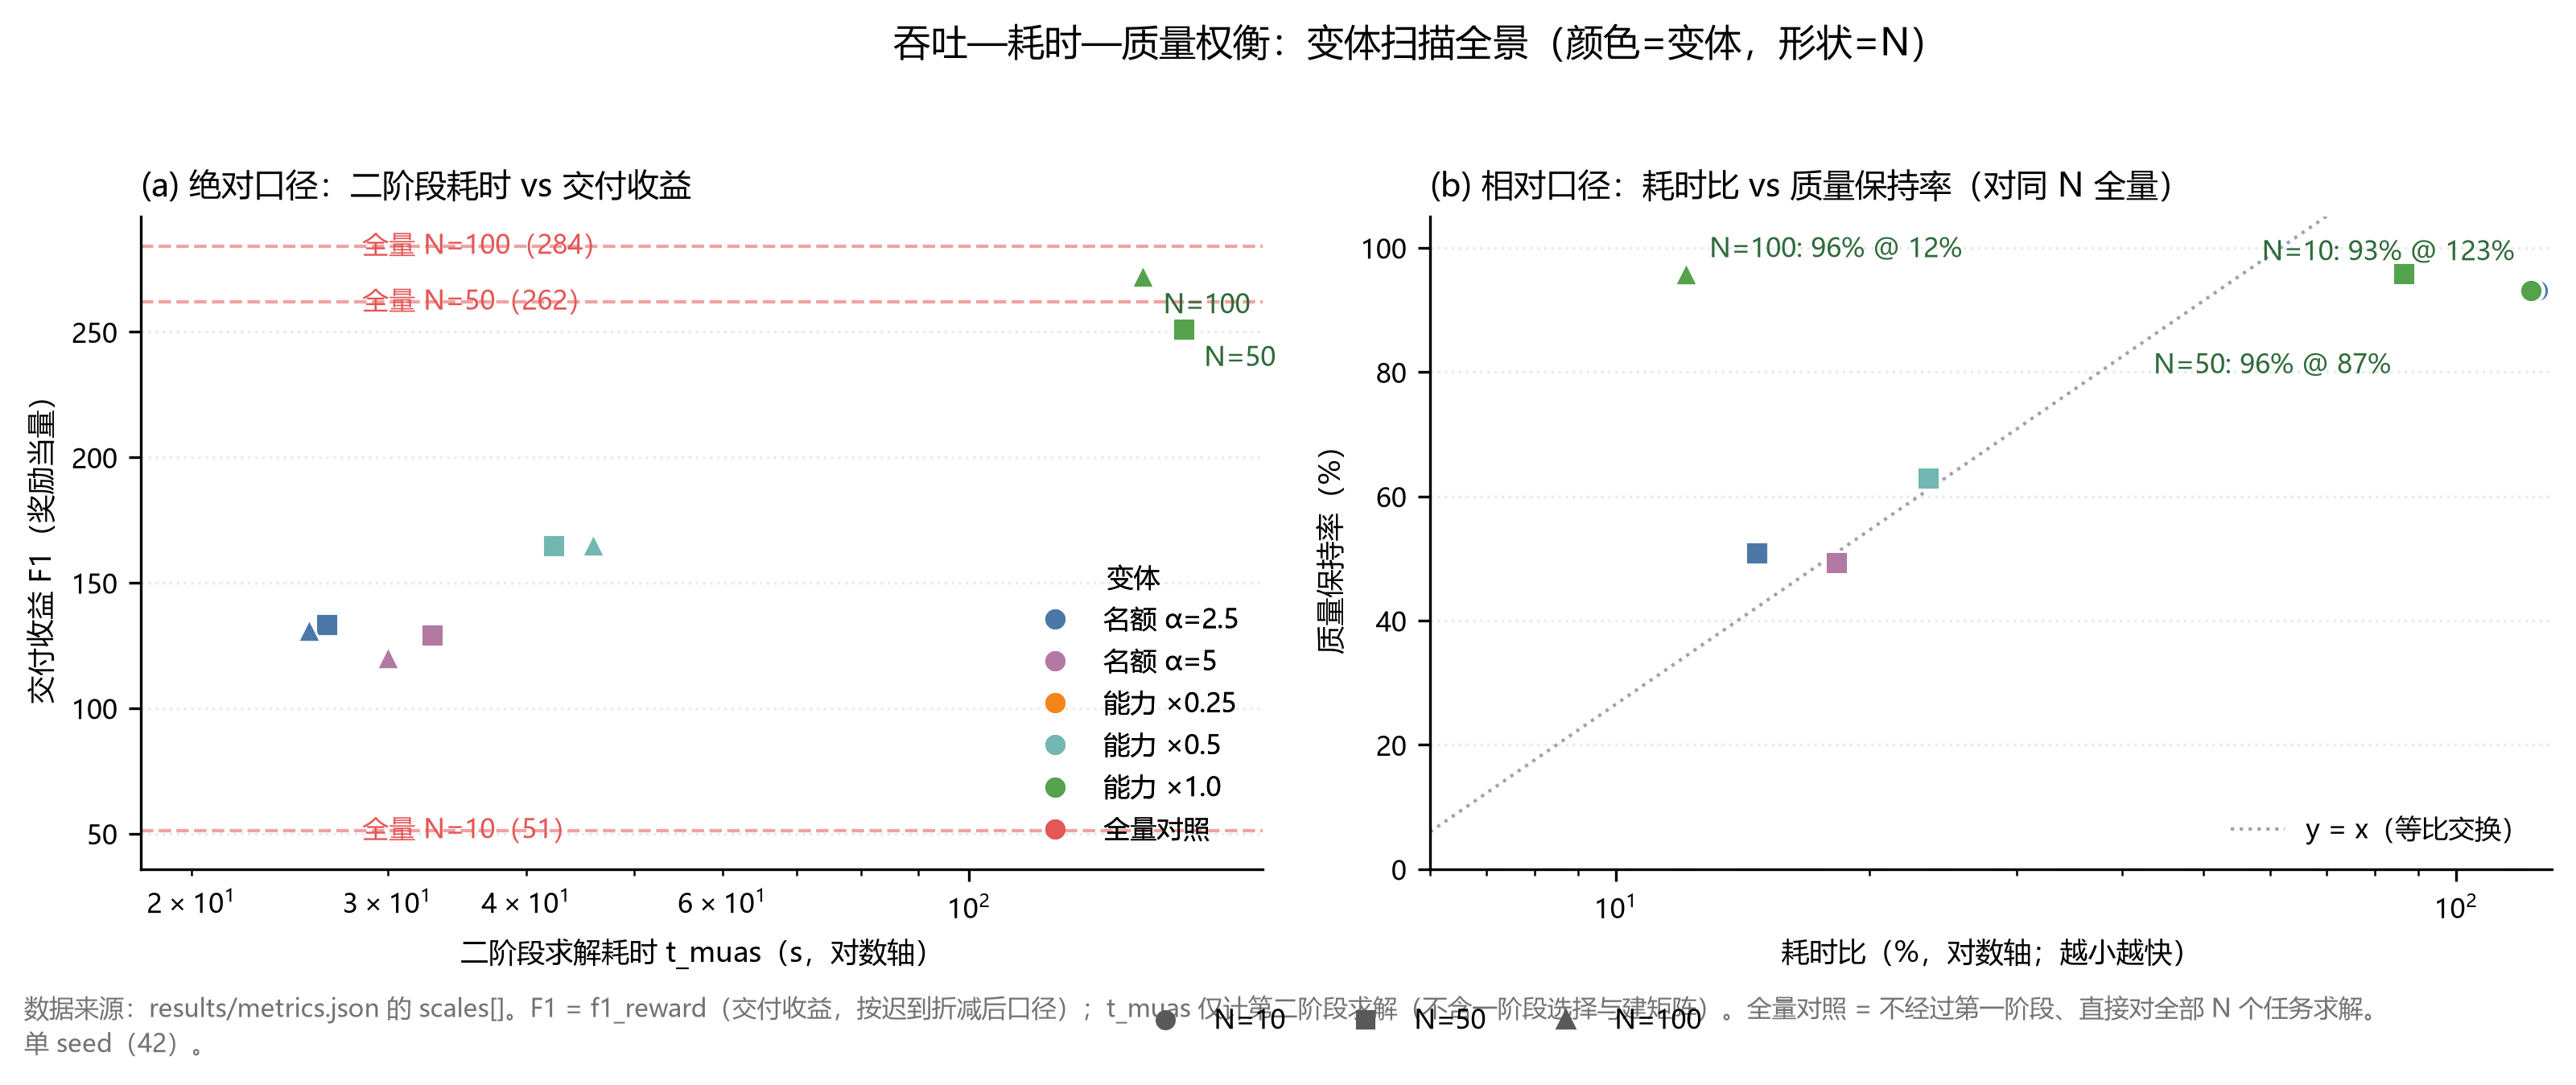
\includegraphics[width=\textwidth]{R01_tradeoff.png}
\caption{吞吐—耗时—质量权衡：全变体扫描全景。(a)~绝对口径：二阶段耗时
（对数轴）vs 交付收益 F1，红色虚线为同 $N$ 全量对照；(b)~相对口径：
耗时比 vs 质量保持率（对同 $N$ 全量），右下为优。能力族（绿/青/橙）沿
「掉质量换耗时」的曲线分布，$n_{\mathrm{sel}} \approx \mathrm{cap}(t)$ 的 \texttt{cap\_x1}
位于曲线拐点；名额族（蓝/紫）全部挤在左上角——质量保持率低且耗时并不更低
（被 $\lceil \mathrm{max\_ratio} \cdot K \rceil = 16$ 封顶）。}
\label{fig:tradeoff}
\end{figure}

\subsection{规模压缩与 N 解耦（成功标准 1）}

\begin{figure}[H]
\centering
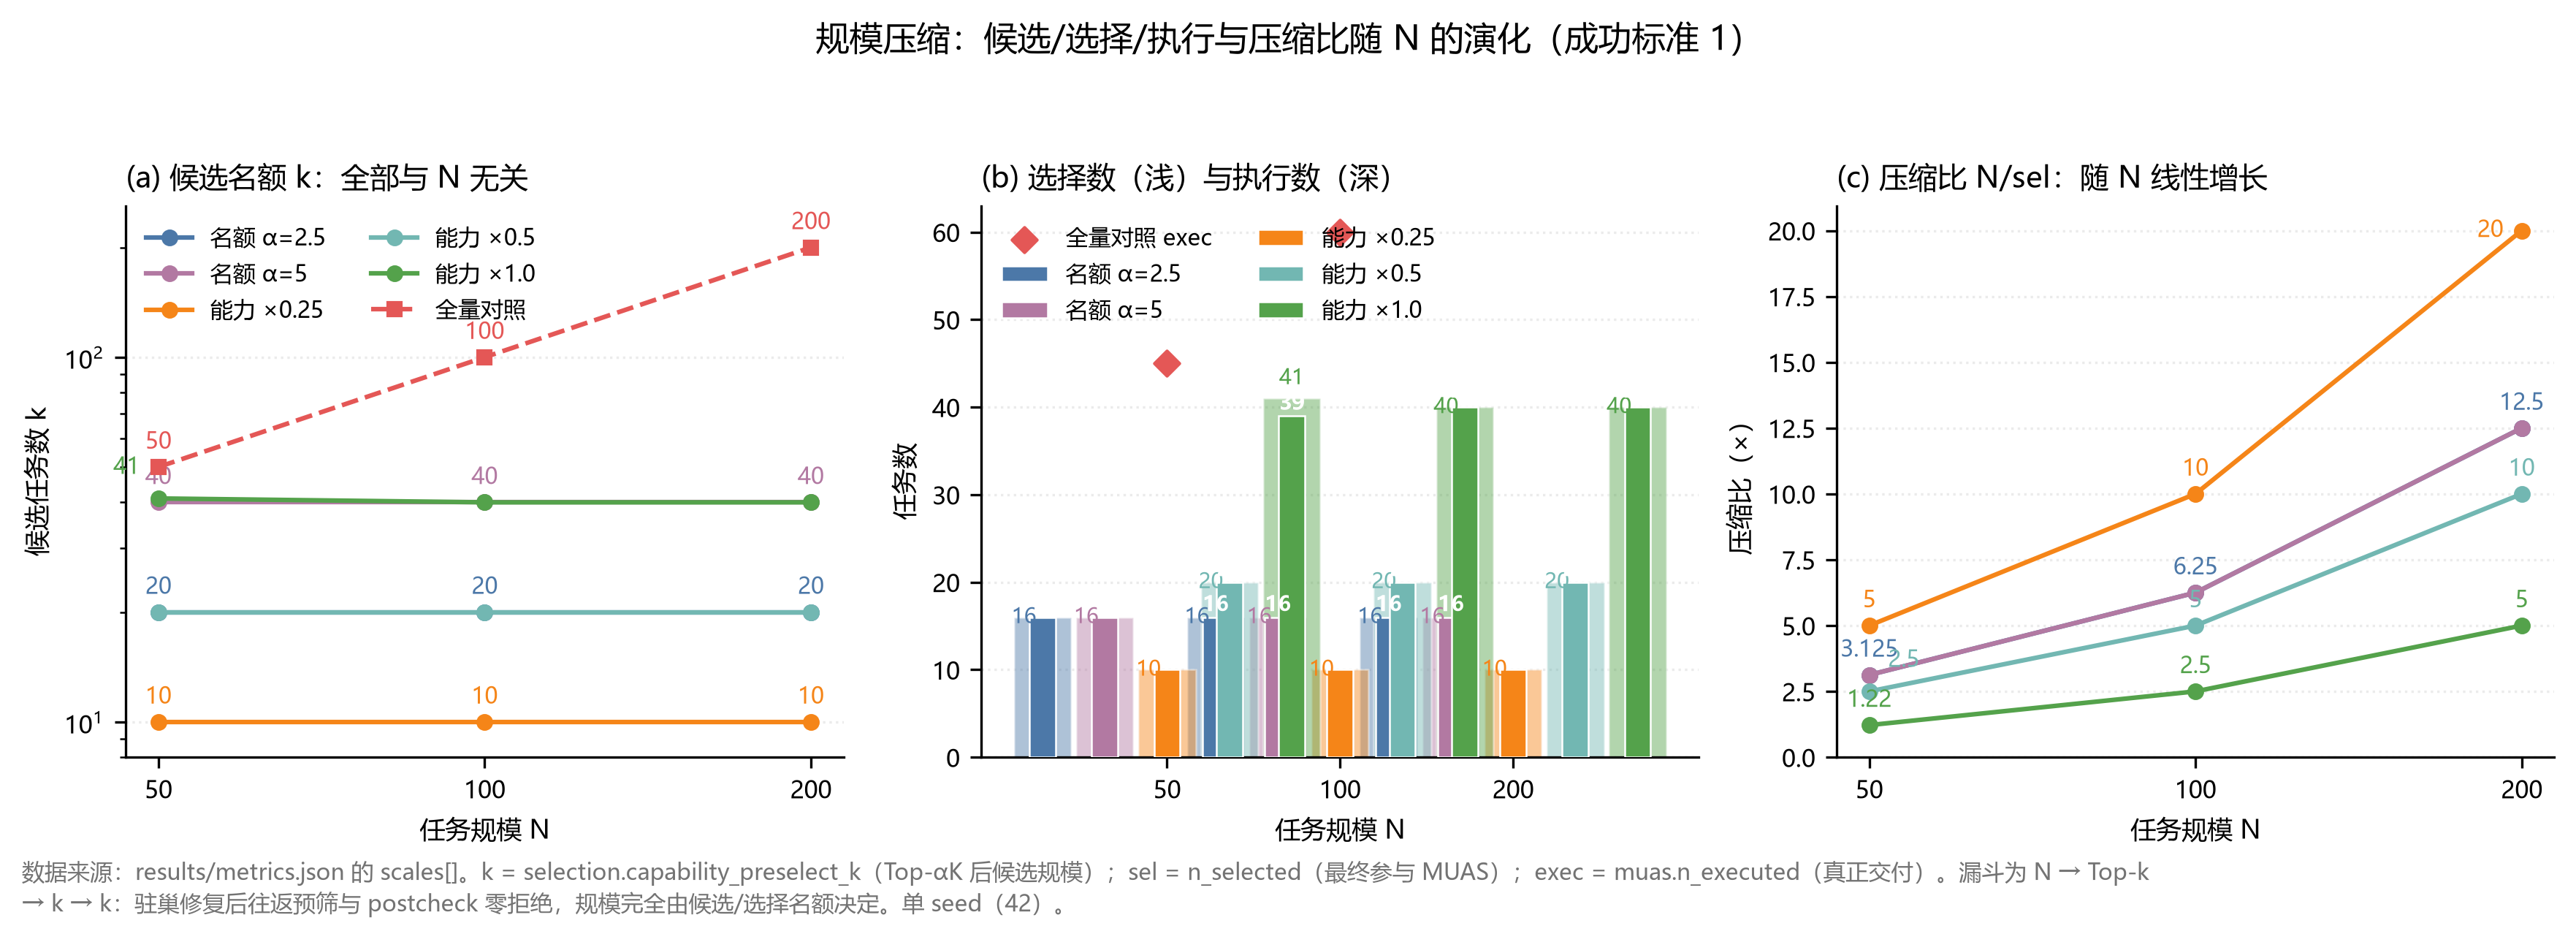
\includegraphics[width=\textwidth]{R02_compression.png}
\caption{规模压缩：候选/选择/执行与压缩比随 $N$ 的演化。
(a)~候选数 $n_{\mathrm{cand}}$ 全部与 $N$ 无关（平线；全量对照为斜线）；
(b)~选择数（浅柱）与执行数（深柱）——漏斗 $N \to n_{\mathrm{cand}} \to n_{\mathrm{sel}} \to \mathrm{exec}$
的末两级；(c)~压缩比随 $N$ 线性增长（名额族 $3.1\times \to 12.5\times$）。}
\label{fig:compression}
\end{figure}

\subsection{耗时分解与惰性边（成功标准 2 + 优化 A 证据）}

\begin{figure}[H]
\centering
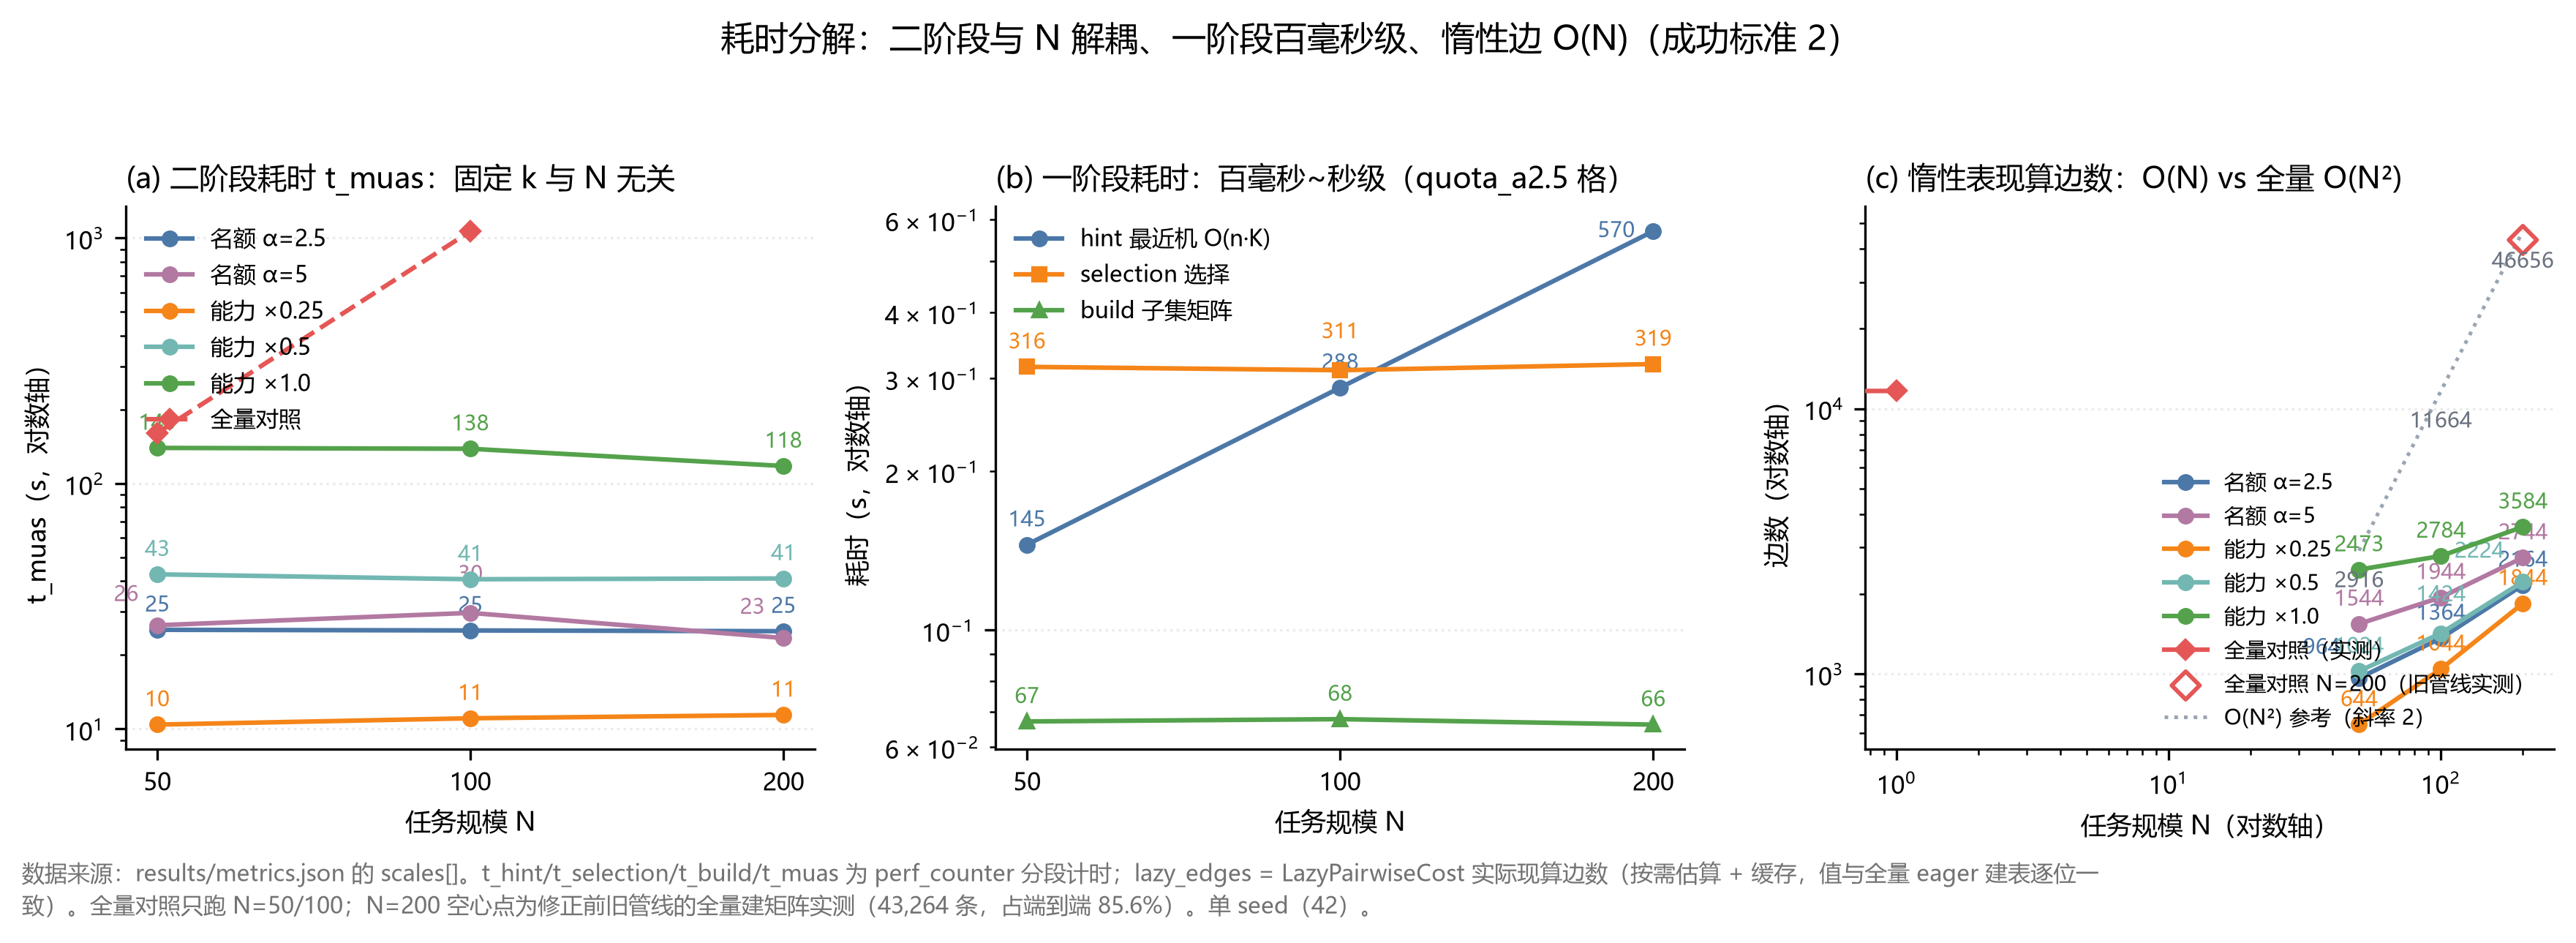
\includegraphics[width=\textwidth]{R03_time_breakdown.png}
\caption{耗时分解。(a)~二阶段耗时固定 $n_{\mathrm{sel}}$ 与 $N$ 无关（$n_{\mathrm{sel}}{=}16$：
25.3/25.2/25.0\,s，极差 $<2\%$）；(b)~一阶段三项耗时全程百毫秒~秒级
（$N{=}200$ 合计 0.96\,s = 端到端 3.7\%）；(c)~惰性表现算边数沿 $O(N)$
增长，全量矩阵沿 $O(N^2)$（斜率 2 参考线），$N{=}200$ 时惰性 2,164 条
= 全量的 5.0\%。}
\label{fig:time}
\end{figure}

\subsection{瓶颈定位：选择数封顶而非候选倍率}

\begin{figure}[H]
\centering
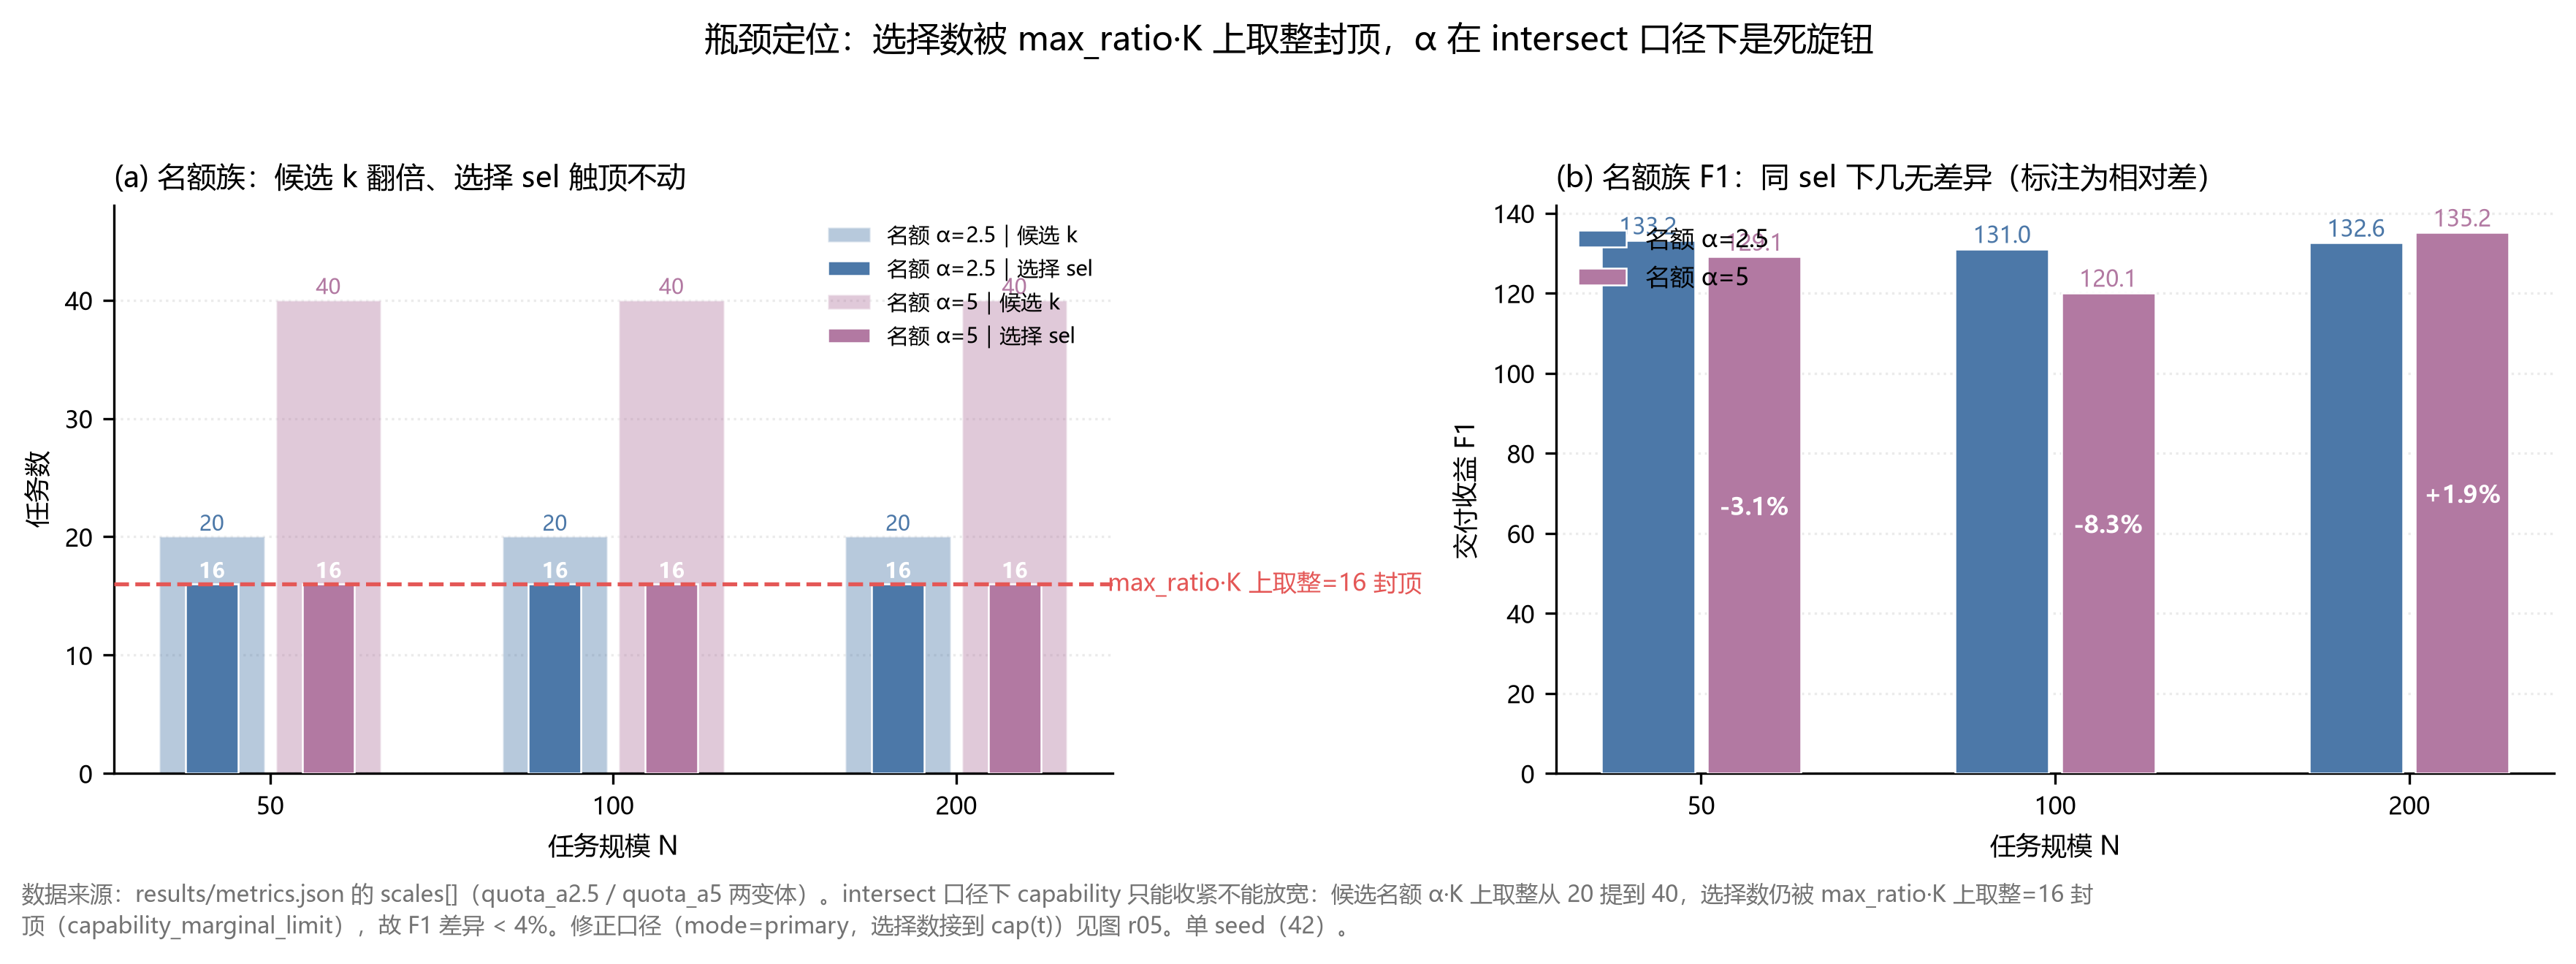
\includegraphics[width=\textwidth]{R04_bottleneck.png}
\caption{瓶颈定位。(a)~名额族候选 $n_{\mathrm{cand}}$ 翻倍（$20 \to 40$）、选择 $n_{\mathrm{sel}}$ 触顶不动
（16/16/16），红色虚线为 $\lceil \mathrm{max\_ratio} \cdot K \rceil = 16$ 封顶线；
(b)~同 $n_{\mathrm{sel}}$ 下两变体 F1 几无差异（标注为相对差，最大 $-8.3\%$）——
候选数在该区间是「死旋钮」。修正口径（选择数接到 $\mathrm{cap}(t)$）见图~\ref{fig:capability}。}
\label{fig:bottleneck}
\end{figure}

\subsection{能力驱动标定：cap(t) 是天然平衡点（成功标准 3/4）}

\begin{figure}[H]
\centering
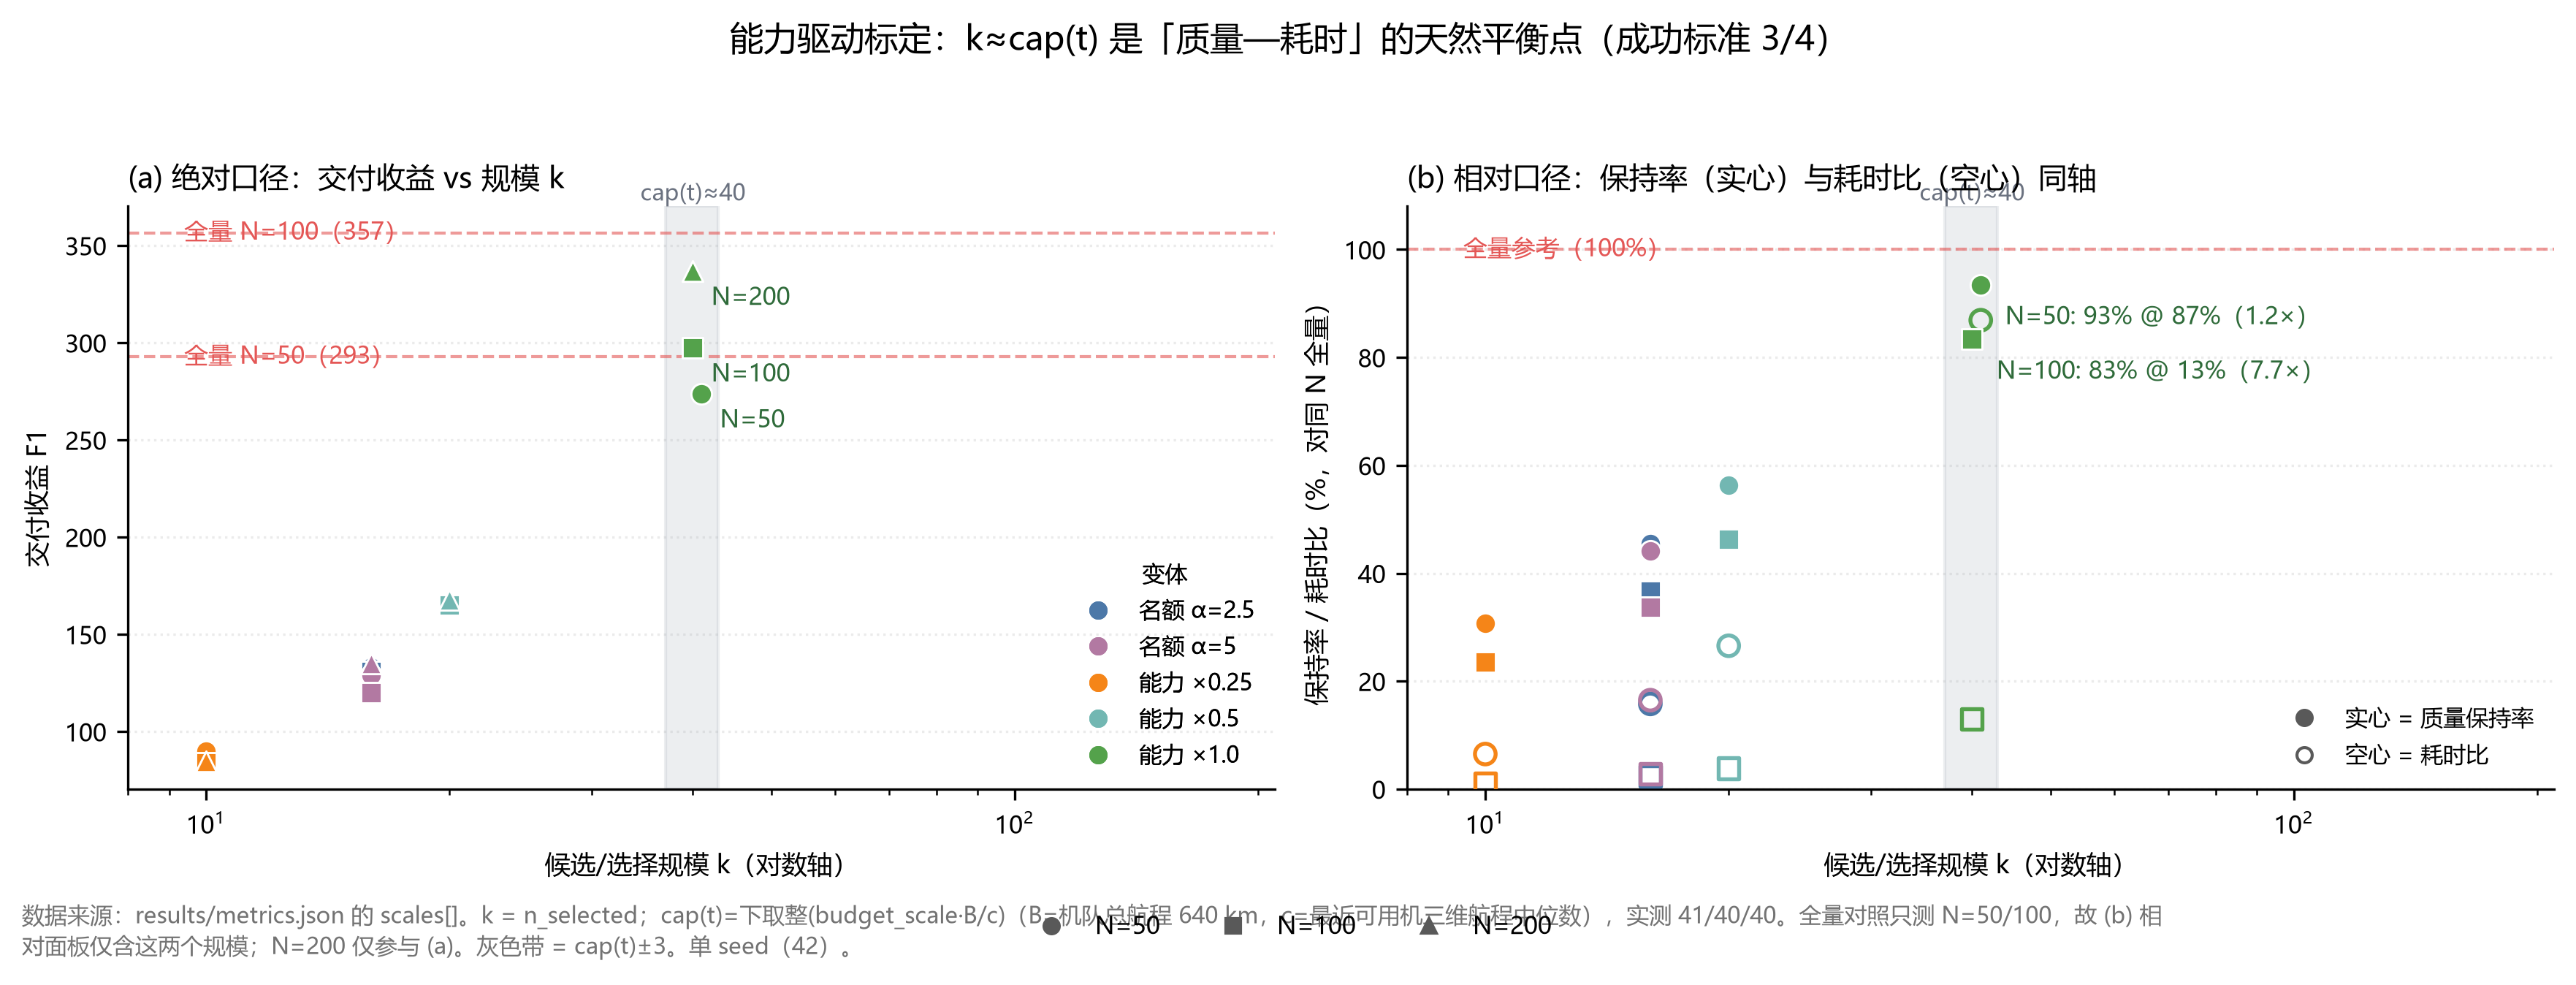
\includegraphics[width=\textwidth]{R05_capability.png}
\caption{能力驱动标定（灰色带 = $\mathrm{cap}(t) \pm 3$）。
(a)~绝对口径：交付收益 vs 规模 $n_{\mathrm{sel}}$，\texttt{cap\_x1}（$n_{\mathrm{sel}} \approx \mathrm{cap}(t) = 40$）
达到全量的 93.5\%（$N{=}50$）/ 83.4\%（$N{=}100$）；
(b)~相对口径：质量保持率（实心）与耗时比（空心）同轴，\texttt{cap\_x1} 在
$N{=}100$ 用 13\% 的耗时拿到 83.4\% 的质量（7.6$\times$ 加速）。
$n_{\mathrm{sel}}$ 从 41 加到 50（全量）只多 7\% F1 却多 16\% 耗时——$\mathrm{cap}(t)$
右侧收益速衰，即「天然平衡点」。}
\label{fig:capability}
\end{figure}

% ============================================================
\section{附：数据与复现}
% ============================================================

\begin{table}[H]
\centering
\caption{数据文件清单（均位于 \texttt{results/}）}
\label{tab:files}
\small
\begin{tabular}{ll}
\toprule
文件 & 内容 \\
\midrule
\texttt{metrics.json} & $N \times$ variant 扫描矩阵（17 格；本报告全部数值来源） \\
\texttt{run\_meta.json} & 运行元数据（实验名、配置路径、时间戳） \\
\texttt{figures/} & 6 个图产物（S01 + R01--R05） \\
\bottomrule
\end{tabular}
\end{table}

复现方式：在本实验目录执行
\fname{python run.py}（默认配置即本报告口径，
\fname{output\_dir: results}；\fname{-{}-no-plots} 可跳过出图）。
求解全部完成后才调 \fname{make\_plots}；若绘图阶段被工具超时打断（600\,s），
用 \fname{python render\_from\_json.py png}（或 \fname{pdf}）按格式/图 id
补出，不必重跑求解——绘图只读 \fname{metrics.json}，与数值产物同源。

单图独立调试：\fname{python plot/report/r01\_tradeoff.py}
（自举转 \fname{-m} 语义，\fname{-{}-pdf} 额外输出矢量图，
\fname{-{}-dpi N} 指定分辨率，\fname{-{}-results DIR} 指定结果目录）。

出图约定（与 exp01\_smoke 同口径）：\fname{plot/registry.py} 是图清单唯一
事实来源（新增图 = 加一行）；\fname{plot/theme.py} 是唯一 import pyplot
的地方（学术字号 8.5\,pt 基、Tableau 10 派生配色、300\,dpi 印刷级）；
出图末端统一执行版面自检（越界 / 文本互压 / 轴标题折行）与自动去重叠。

\end{document}
